% ============================================================
% VISTA-MPC + SARL: Vision-Language Informed Socially Attentive
% Model Predictive Control for Robot Navigation
% ============================================================
\documentclass[aspectratio=169, 10pt]{beamer}

% ---- Packages ----
\usepackage[utf8]{inputenc}
\usepackage[T1]{fontenc}
\usepackage{amsmath, amssymb, amsfonts}
\usepackage{mathtools}
\usepackage{bm}
\usepackage{tikz}
\usetikzlibrary{
  arrows.meta, positioning, shapes.geometric, shapes.misc,
  fit, calc, decorations.pathreplacing, backgrounds,
  matrix, chains
}
\usepackage{booktabs}
\usepackage{multirow}
\usepackage{algorithm}
\usepackage{algorithmic}
\usepackage{graphicx}
\usepackage{xcolor}
\usepackage{hyperref}
\usepackage{appendixnumberbeamer}

% ---- Theme Configuration ----
\usetheme{Madrid}
\usecolortheme{whale}
\usefonttheme{professionalfonts}

% Custom colors
\definecolor{sarlblue}{RGB}{41, 98, 255}
\definecolor{vlmgreen}{RGB}{0, 150, 80}
\definecolor{mpcred}{RGB}{200, 40, 40}
\definecolor{synergyorange}{RGB}{230, 130, 0}
\definecolor{lightbg}{RGB}{245, 248, 255}
\definecolor{darktext}{RGB}{30, 30, 50}
\definecolor{attentionhigh}{RGB}{220, 50, 50}
\definecolor{attentionlow}{RGB}{50, 180, 80}

\setbeamercolor{frametitle}{bg=sarlblue!90!black, fg=white}
\setbeamercolor{title}{bg=sarlblue!90!black, fg=white}
\setbeamercolor{structure}{fg=sarlblue}
\setbeamercolor{block title}{bg=sarlblue!80, fg=white}
\setbeamercolor{block body}{bg=sarlblue!5}
\setbeamercolor{block title alerted}{bg=mpcred!80, fg=white}
\setbeamercolor{block body alerted}{bg=mpcred!5}
\setbeamercolor{block title example}{bg=vlmgreen!70, fg=white}
\setbeamercolor{block body example}{bg=vlmgreen!5}

% Remove navigation symbols
\setbeamertemplate{navigation symbols}{}

% Page numbering
\setbeamertemplate{footline}{
  \hfill
  \usebeamercolor[fg]{page number in head/foot}
  \usebeamerfont{page number in head/foot}
  \insertframenumber\,/\,\inserttotalframenumber\kern1.5em\vskip4pt
}

% Custom commands
\newcommand{\highlight}[1]{\textcolor{sarlblue}{\textbf{#1}}}
\newcommand{\vlmhl}[1]{\textcolor{vlmgreen}{\textbf{#1}}}
\newcommand{\mpchl}[1]{\textcolor{mpcred}{\textbf{#1}}}
\newcommand{\synhl}[1]{\textcolor{synergyorange}{\textbf{#1}}}
\setbeamertemplate{blocks}[rounded][shadow=false]
% Math operators
\DeclareMathOperator*{\argmin}{arg\,min}
\DeclareMathOperator{\softmax}{softmax}

% ============================================================
% TITLE PAGE
% ============================================================
\title[VISTA-MPC + SARL]{%
  \textbf{VISTA-MPC}\\[4pt]
  \large Vision-Language Informed Socially Attentive\\
  Model Predictive Control for Robot Navigation}

\author{Jiaxi Huo}

\institute{University of Technology Sydney}

\date{\today}

\begin{document}

% ---- Title Frame ----
\begin{frame}[plain]
  \titlepage
\end{frame}

% ---- Outline ----
\begin{frame}{Outline}
  \tableofcontents
\end{frame}

% ============================================================
\section{Motivation}
% ============================================================

\begin{frame}{The Challenge of Social Robot Navigation}
  \begin{columns}[T]
    \begin{column}{0.55\textwidth}
      \textbf{Problem:} Robots navigating in human-populated environments must respect
      \emph{implicit social norms}, not just avoid collisions.

      \vspace{6pt}
      \textbf{Key challenges:}
      \begin{itemize}
        \item Variable crowd density and scene structure
        \item Not all pedestrians are equally important
        \item Context-dependent social behavior \\
              (doorway $\neq$ open space)
        \item Real-time control under uncertainty
        \item Need for \emph{interpretable} decisions
      \end{itemize}

      \vspace{6pt}
      \textbf{Our Insight:}
      Combine \highlight{learned social attention} (SARL),
      \vlmhl{scene understanding} (VLM), and
      \mpchl{optimal control} (MPC) in a principled hierarchy.
    \end{column}
    \begin{column}{0.42\textwidth}
      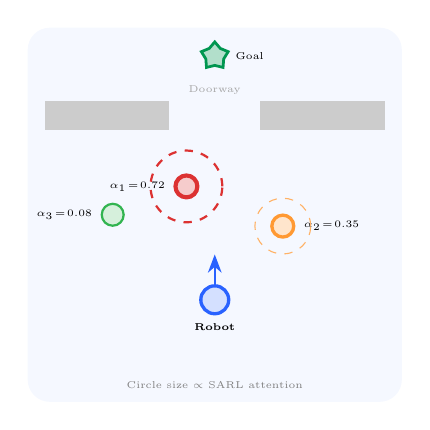
\begin{tikzpicture}[
        scale=0.72, transform shape,
        every node/.style={font=\small}
      ]
        % Scene background
        \fill[lightbg, rounded corners=8pt] (-0.3,-0.3) rectangle (6.3,6.3);

        % Walls (doorway scenario)
        \fill[gray!40] (0,4.5) rectangle (2.2,5.0);
        \fill[gray!40] (3.8,4.5) rectangle (6,5.0);
        \node[font=\tiny, gray!70] at (3,5.2) {Doorway};

        % Robot
        \node[circle, draw=sarlblue, fill=sarlblue!20,
              minimum size=14pt, line width=1.2pt] (robot) at (3,1.5) {};
        \node[font=\tiny, below=1pt of robot] {\textbf{Robot}};
        \draw[-{Stealth}, sarlblue, thick] (robot) -- ++(0,0.8);

        % Goal
        \node[star, star points=5, draw=vlmgreen, fill=vlmgreen!30,
              minimum size=10pt, line width=1pt] (goal) at (3,5.8) {};
        \node[font=\tiny, right=1pt of goal] {Goal};

        % Pedestrians with different attention
        \node[circle, draw=attentionhigh, fill=attentionhigh!25,
              minimum size=11pt, line width=1.5pt] (p1) at (2.5,3.5) {};
        \node[font=\tiny, left=1pt of p1] {$\alpha_1\!=\!0.72$};

        \node[circle, draw=orange!80, fill=orange!20,
              minimum size=11pt, line width=1.2pt] (p2) at (4.2,2.8) {};
        \node[font=\tiny, right=1pt of p2] {$\alpha_2\!=\!0.35$};

        \node[circle, draw=attentionlow, fill=attentionlow!20,
              minimum size=11pt, line width=0.8pt] (p3) at (1.2,3.0) {};
        \node[font=\tiny, left=1pt of p3] {$\alpha_3\!=\!0.08$};

        % Attention rings
        \draw[attentionhigh, dashed, thick] (p1) circle (18pt);
        \draw[orange!60, dashed] (p2) circle (14pt);

        % Legend
        \node[font=\tiny, text=gray] at (3,0) {Circle size $\propto$ SARL attention};
      \end{tikzpicture}
    \end{column}
  \end{columns}
\end{frame}

% ============================================================
\begin{frame}{Limitations of Existing Approaches}
  \begin{columns}[T]
    \begin{column}{0.48\textwidth}
      \begin{alertblock}{Reactive Methods (DWA, RVO2)}
        \begin{itemize}
          \item[\textcolor{mpcred}{\scriptsize$\blacksquare$}] Treat all pedestrians equally
          \item[\textcolor{mpcred}{\scriptsize$\blacksquare$}] No scene context understanding
          \item[\textcolor{mpcred}{\scriptsize$\blacksquare$}] Myopic --- no lookahead
        \end{itemize}
      \end{alertblock}

      \vspace{4pt}
      \begin{alertblock}{End-to-End RL}
        \begin{itemize}
          \item[\textcolor{mpcred}{\scriptsize$\blacksquare$}] Black-box decisions
          \item[\textcolor{mpcred}{\scriptsize$\blacksquare$}] Sim-to-real transfer gap
          \item[\textcolor{mpcred}{\scriptsize$\blacksquare$}] No safety guarantees
        \end{itemize}
      \end{alertblock}
    \end{column}

    \begin{column}{0.48\textwidth}
      \begin{exampleblock}{VISTA-MPC + SARL (Ours)}
        \begin{itemize}
          \item[\textcolor{vlmgreen}{\scriptsize$\blacksquare$}] \textbf{Attention-weighted} social reasoning
          \item[\textcolor{vlmgreen}{\scriptsize$\blacksquare$}] \textbf{Scene-adaptive} via VLM
          \item[\textcolor{vlmgreen}{\scriptsize$\blacksquare$}] \textbf{Predictive} MPC horizon (3\,s)
          \item[\textcolor{vlmgreen}{\scriptsize$\blacksquare$}] \textbf{Interpretable} explanations
          \item[\textcolor{vlmgreen}{\scriptsize$\blacksquare$}] \textbf{Safety guarantees} via hard constraints
          \item[\textcolor{vlmgreen}{\scriptsize$\blacksquare$}] \textbf{Graceful fallback} when data stale
        \end{itemize}
      \end{exampleblock}
    \end{column}
  \end{columns}

  \vspace{8pt}
  \centering
  
\begin{tikzpicture}
    \node[draw=synergyorange, fill=synergyorange!8, rounded corners=6pt,
          text width=0.85\textwidth, align=center, font=\small,
          line width=1pt] {
      \synhl{Key Idea:} Use RL for \emph{what to attend to},
      VLM for \emph{scene understanding},
      and MPC for \emph{safe optimal control}.
    };
  \end{tikzpicture}
\end{frame}

% ============================================================
\section{System Architecture}
% ============================================================

\begin{frame}{Three-Layer Hierarchical Architecture}
  \centering
  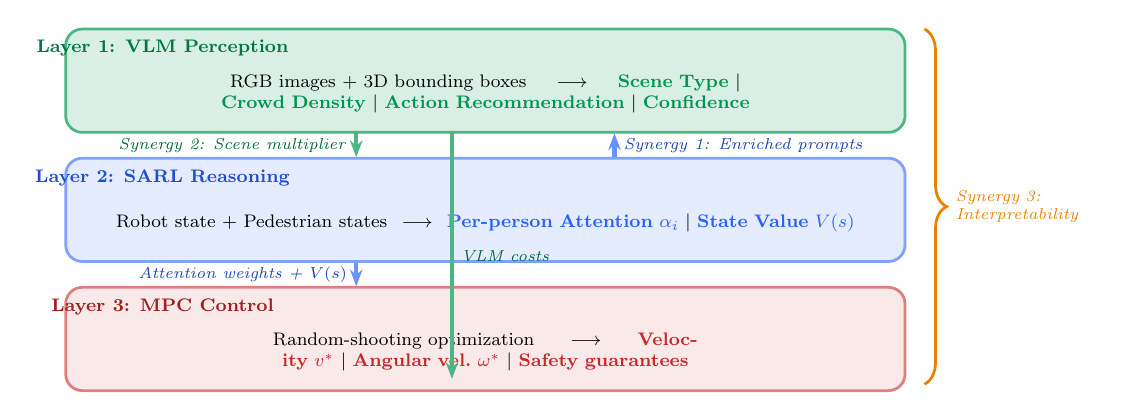
\begin{tikzpicture}[
    scale=0.82, transform shape,
    layer/.style={draw, rounded corners=6pt, minimum width=13cm,
                  minimum height=1.6cm, align=center, font=\small,
                  line width=1pt},
    arrow/.style={-{Stealth[length=6pt]}, thick},
    lbl/.style={font=\footnotesize\bfseries, text=white},
  ]
    % Layer 3: VLM (top)
    \node[layer, fill=vlmgreen!15, draw=vlmgreen!70] (vlm) at (0,4.2) {};
    \node[lbl, text=vlmgreen!80!black] at (-5, 4.7) {Layer 1: VLM Perception};
    \node[font=\footnotesize, text width=12cm, align=center] at (0,4.0) {
      RGB images + 3D bounding boxes $\;\longrightarrow\;$
      \vlmhl{Scene Type} \textbar{} \vlmhl{Crowd Density} \textbar{}
      \vlmhl{Action Recommendation} \textbar{} \vlmhl{Confidence}
    };

    % Layer 2: SARL (middle)
    \node[layer, fill=sarlblue!12, draw=sarlblue!60] (sarl) at (0,2.2) {};
    \node[lbl, text=sarlblue!80!black] at (-5, 2.7) {Layer 2: SARL Reasoning};
    \node[font=\footnotesize, text width=12cm, align=center] at (0,2.0) {
      Robot state + Pedestrian states $\;\longrightarrow\;$
      \highlight{Per-person Attention $\alpha_i$} \textbar{}
      \highlight{State Value $V(s)$}
    };

    % Layer 3: MPC (bottom)
    \node[layer, fill=mpcred!10, draw=mpcred!60] (mpc) at (0,0.2) {};
    \node[lbl, text=mpcred!80!black] at (-5, 0.7) {Layer 3: MPC Control};
    \node[font=\footnotesize, text width=12cm, align=center] at (0,0.0) {
      Random-shooting optimization $\;\longrightarrow\;$
      \mpchl{Velocity $v^*$} \textbar{} \mpchl{Angular vel.\ $\omega^*$}
      \textbar{} \mpchl{Safety guarantees}
    };

    % Synergy arrows
    \draw[arrow, vlmgreen!70, line width=1.5pt]
      ([xshift=-2cm]vlm.south) -- ([xshift=-2cm]sarl.north)
      node[midway, left, font=\scriptsize, text=vlmgreen!70!black]
      {\textit{Synergy 2: Scene multiplier}};

    \draw[arrow, sarlblue!70, line width=1.5pt]
      ([xshift=-2cm]sarl.south) -- ([xshift=-2cm]mpc.north)
      node[midway, left, font=\scriptsize, text=sarlblue!70!black]
      {\textit{Attention weights + $V(s)$}};

    \draw[arrow, sarlblue!70, line width=1.5pt]
      ([xshift=2cm]sarl.north) -- ([xshift=2cm]vlm.south)
      node[midway, right, font=\scriptsize, text=sarlblue!70!black]
      {\textit{Synergy 1: Enriched prompts}};

    \draw[arrow, vlmgreen!70, line width=1.5pt]
      ([xshift=2cm]vlm.south west) ++(4,0) -- ++(0,-3.8)
      node[midway, right, font=\scriptsize, text=vlmgreen!70!black]
      {\textit{VLM costs}};

    % Synergy 3 bracket
    \draw[decorate, decoration={brace, amplitude=8pt, mirror},
          synergyorange, line width=1pt]
      (6.8, -0.5) -- (6.8, 5.0)
      node[midway, right=10pt, font=\scriptsize, text=synergyorange,
           text width=2cm, align=left] {\textit{Synergy 3:\\Interpretability}};
  \end{tikzpicture}
\end{frame}

% ============================================================
\section{SARL: Socially Attentive Reinforcement Learning}
% ============================================================

\begin{frame}{SARL Value Network Architecture}
  \centering
  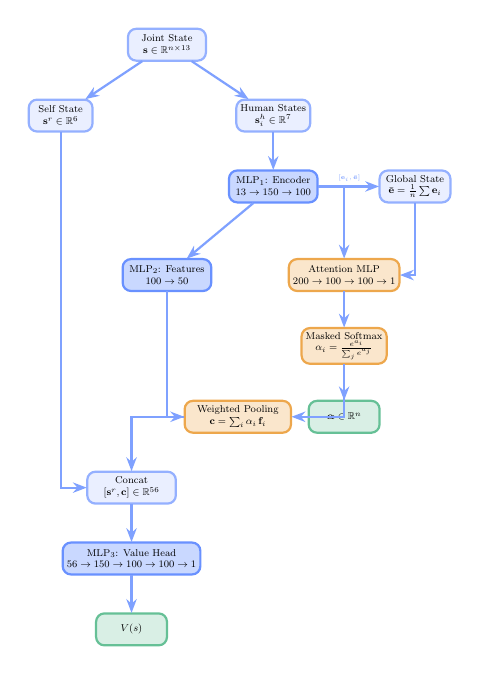
\begin{tikzpicture}[
    scale=0.45, transform shape,
    box/.style={draw, rounded corners=3pt, minimum height=0.9cm,
                align=center, font=\footnotesize, line width=0.8pt},
    data/.style={box, fill=sarlblue!10, draw=sarlblue!50,
                 minimum width=2.2cm},
    mlp/.style={box, fill=sarlblue!25, draw=sarlblue!70,
                minimum width=2.5cm},
    attn/.style={box, fill=synergyorange!20, draw=synergyorange!70,
                 minimum width=2.5cm},
    outputbox/.style={box, fill=vlmgreen!15, draw=vlmgreen!60,
                minimum width=2cm},
    arrow/.style={-{Stealth[length=5pt]}, thick, sarlblue!60},
  ]
    % Input
    \node[data] (input) at (0,0) {Joint State\\$\mathbf{s} \in \mathbb{R}^{n \times 13}$};

    % Self state split
    \node[data, minimum width=1.8cm] (self) at (-3,-2) {Self State\\$\mathbf{s}^r \in \mathbb{R}^6$};
    \node[data, minimum width=1.8cm] (human) at (3,-2) {Human States\\$\mathbf{s}^h_i \in \mathbb{R}^7$};

    % MLP1
    \node[mlp] (mlp1) at (3,-4) {MLP$_1$: Encoder\\$13 \to 150 \to 100$};

    % Global state
    \node[data, minimum width=2cm] (global) at (7,-4) {Global State\\$\bar{\mathbf{e}} = \frac{1}{n}\sum \mathbf{e}_i$};

    % Attention
    \node[attn] (attn) at (5,-6.5) {Attention MLP\\$200 \to 100 \to 100 \to 1$};

    % Softmax
    \node[attn, minimum width=2cm] (softmax) at (5,-8.5) {Masked Softmax\\$\alpha_i = \frac{e^{a_i}}{\sum_j e^{a_j}}$};

    % MLP2
    \node[mlp] (mlp2) at (0,-6.5) {MLP$_2$: Features\\$100 \to 50$};

    % Weighted sum
    \node[attn, minimum width=3cm] (wsum) at (2,-10.5) {Weighted Pooling\\$\mathbf{c} = \sum_i \alpha_i \, \mathbf{f}_i$};

    % Concatenate
    \node[data, minimum width=2.5cm] (concat) at (-1,-12.5) {Concat\\$[\mathbf{s}^r, \mathbf{c}] \in \mathbb{R}^{56}$};

    % MLP3
    \node[mlp] (mlp3) at (-1,-14.5) {MLP$_3$: Value Head\\$56 \to 150 \to 100 \to 100 \to 1$};

    % Output
    \node[outputbox] (vout) at (-1,-16.5) {$V(s)$};
    \node[outputbox] (aout) at (5,-10.5) {$\bm{\alpha} \in \mathbb{R}^n$};

    % Arrows
    \draw[arrow] (input) -- (self);
    \draw[arrow] (input) -- (human);
    \draw[arrow] (human) -- (mlp1);
    \draw[arrow] (mlp1) -- (global);
    \draw[arrow] (mlp1) -- (mlp2);
    \draw[arrow] (mlp1) -| node[above right, font=\tiny, pos=0.3] {$[\mathbf{e}_i, \bar{\mathbf{e}}]$} (attn);
    \draw[arrow] (global) |- (attn);
    \draw[arrow] (attn) -- (softmax);
    \draw[arrow] (softmax) -- (aout);
    \draw[arrow] (softmax) |- (wsum);
    \draw[arrow] (mlp2) |- (wsum);
    \draw[arrow] (wsum) -| (concat);
    \draw[arrow] (self) |- (concat);
    \draw[arrow] (concat) -- (mlp3);
    \draw[arrow] (mlp3) -- (vout);
  \end{tikzpicture}
\end{frame}

% ============================================================
\begin{frame}{SARL: State Representation \& Coordinate Transform}
  \begin{columns}[T]
    \begin{column}{0.52\textwidth}
      \textbf{Joint State Vector} (per human $i$):
      \[
        \mathbf{s}_i = \bigl[\underbrace{d_g,\; v_{\text{pref}},\; \theta,\; r}_{\text{self state}},\;
        \underbrace{v_x^r,\; v_y^r}_{\text{velocity}},\;
        \underbrace{p_x^i,\; p_y^i,\; v_x^i,\; v_y^i,\; r^i,\; d_a,\; r_{\Sigma}}_{\text{human state}}\bigr]
      \]

      \vspace{4pt}
      \textbf{Goal-Oriented Rotation:}
      \[
        \theta_{\text{rot}} = \text{atan2}(g_y - p_y^r,\; g_x - p_x^r)
      \]
      \[
        \mathbf{R} = \begin{bmatrix}
          \cos\theta_{\text{rot}} & \sin\theta_{\text{rot}} \\
          -\sin\theta_{\text{rot}} & \cos\theta_{\text{rot}}
        \end{bmatrix}
      \]

      \vspace{4pt}
      Applied to all velocity and position vectors:
      \[
        \mathbf{v}_{\text{rot}} = \mathbf{R}\,\mathbf{v}_{\text{world}}, \quad
        \mathbf{p}_{\text{rot}}^i = \mathbf{R}\,(\mathbf{p}_{\text{world}}^i - \mathbf{p}^r)
      \]
    \end{column}

    \begin{column}{0.45\textwidth}
      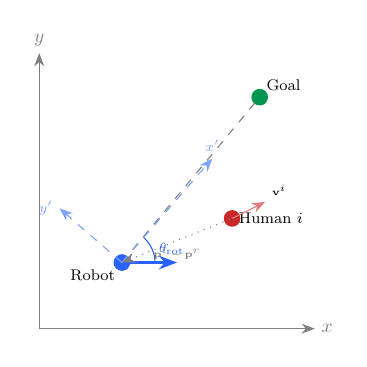
\begin{tikzpicture}[scale=0.7, transform shape]
        % Coordinate axes
        \draw[-{Stealth}, gray] (0,0) -- (5,0) node[right] {$x$};
        \draw[-{Stealth}, gray] (0,0) -- (0,5) node[above] {$y$};

        % Robot
        \filldraw[sarlblue] (1.5,1.2) circle (4pt);
        \node[font=\footnotesize, below left] at (1.5,1.2) {Robot};

        % Goal
        \filldraw[vlmgreen] (4,4.2) circle (4pt);
        \node[font=\footnotesize, above right] at (4,4.2) {Goal};

        % Rotation angle
        \draw[dashed, gray] (1.5,1.2) -- (4,4.2);
        \draw[-{Stealth}, sarlblue, thick] (1.5,1.2) -- (2.5,1.2);
        \draw[sarlblue] (2.1,1.2) arc[start angle=0, end angle=49, radius=0.6]
          node[midway, right, font=\scriptsize] {$\theta_{\text{rot}}$};

        % Rotated axes
        \draw[-{Stealth}, sarlblue!60, dashed] (1.5,1.2) -- ++(49:2.5)
          node[above, font=\scriptsize] {$x'$};
        \draw[-{Stealth}, sarlblue!60, dashed] (1.5,1.2) -- ++(139:1.5)
          node[left, font=\scriptsize] {$y'$};

        % Human
        \filldraw[mpcred] (3.5,2.0) circle (4pt);
        \node[font=\footnotesize, right] at (3.5,2.0) {Human $i$};
        \draw[-{Stealth}, mpcred!60] (3.5,2.0) -- ++(0.6,0.3);
        \node[font=\tiny, above right] at (4.1,2.3) {$\mathbf{v}^i$};

        % Relative position
        \draw[{Stealth}-, dotted, gray] (1.5,1.2) -- (3.5,2.0)
          node[midway, below, font=\tiny] {$\mathbf{p}^i - \mathbf{p}^r$};
      \end{tikzpicture}

      \vspace{6pt}
      \begin{block}{\footnotesize Why Rotate?}
        \footnotesize
        Goal-centric frame makes the policy \emph{translation and rotation invariant} --- the same network weights generalize across positions.
      \end{block}
    \end{column}
  \end{columns}
\end{frame}

% ============================================================
\begin{frame}{Self-Attention Mechanism}
\scriptsize
  \begin{columns}[T]
    \begin{column}{0.55\textwidth}
      \textbf{Stage 1:} Encode each human--robot pair:
      \[
        \mathbf{e}_i = \text{MLP}_1(\mathbf{s}_i) \in \mathbb{R}^{100}
      \]

      \textbf{Stage 2:} Compute global context:
      \[
        \bar{\mathbf{e}} = \frac{1}{n}\sum_{i=1}^{n} \mathbf{e}_i
      \]

      \textbf{Stage 3:} Attention scores with global state:
      \[
        a_i = \text{MLP}_{\text{attn}}\bigl([\mathbf{e}_i,\; \bar{\mathbf{e}}]\bigr) \in \mathbb{R}
      \]

      \textbf{Stage 4:} Masked softmax normalization:
      \[
        \alpha_i = \frac{\exp(a_i) \cdot \mathbb{1}[\mathbf{s}^h_i \neq \mathbf{0}]}
                       {\sum_{j=1}^{n} \exp(a_j) \cdot \mathbb{1}[\mathbf{s}^h_j \neq \mathbf{0}]}
      \]

      \textbf{Stage 5:} Weighted feature aggregation:
      \[
        \mathbf{c} = \sum_{i=1}^{n} \alpha_i \cdot \text{MLP}_2(\mathbf{e}_i) \in \mathbb{R}^{50}
      \]
    \end{column}

    \begin{column}{0.42\textwidth}
      \begin{block}{Interpretation}
        \begin{itemize}
          \item $\alpha_i$ captures \emph{behavioral importance} of pedestrian $i$
          \item Not just proximity --- considers velocity, heading, relative position
          \item Zero-masking handles variable crowd sizes
          \item Global state $\bar{\mathbf{e}}$ provides crowd context to each attention score
        \end{itemize}
      \end{block}

      % \vspace{4pt}
      \begin{exampleblock}{Value Function}
        \[
          V(s) = \text{MLP}_3\bigl([\mathbf{s}^r,\; \mathbf{c}]\bigr) \in \mathbb{R}
        \]
        \vspace{-4pt}
        \begin{itemize}
          \item[\textcolor{vlmgreen}{\scriptsize$\blacksquare$}] Encodes long-term navigation quality
          \item[\textcolor{vlmgreen}{\scriptsize$\blacksquare$}] Used as MPC terminal cost
        \end{itemize}
      \end{exampleblock}
    \end{column}
  \end{columns}
\end{frame}

% ============================================================
\begin{frame}{Two-Phase Training Pipeline}
  \centering
  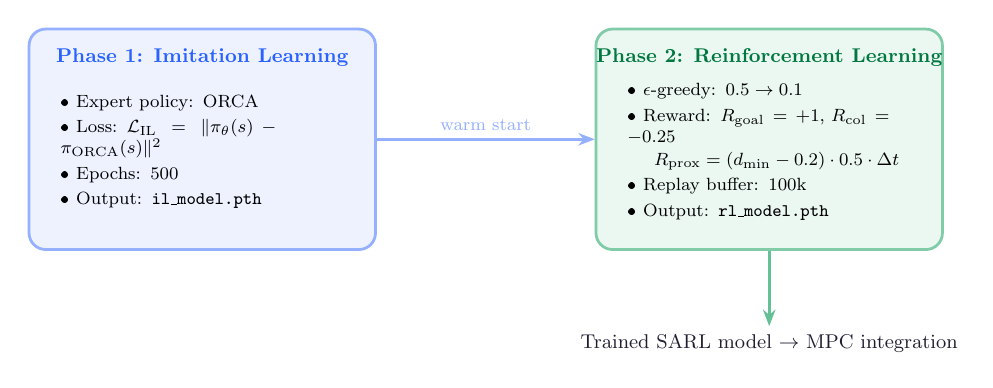
\begin{tikzpicture}[
    scale=0.8, transform shape,
    phase/.style={draw, rounded corners=6pt, minimum width=5.5cm,
                  minimum height=3.5cm, align=center, font=\small,
                  line width=1pt},
    stepbox/.style={font=\footnotesize, align=left},
    arrow/.style={-{Stealth[length=6pt]}, very thick},
  ]
    % Phase 1
    \node[phase, fill=sarlblue!8, draw=sarlblue!50] (il) at (-4.5,0) {};
    \node[font=\small\bfseries, text=sarlblue] at (-4.5,1.3)
      {Phase 1: Imitation Learning};
    \node[stepbox, text width=4.5cm] at (-4.5,-0.2) {
      \textbullet~Expert policy: ORCA\\[2pt]
      \textbullet~Loss: $\mathcal{L}_{\text{IL}} = \|\pi_\theta(s) - \pi_{\text{ORCA}}(s)\|^2$\\[2pt]
      \textbullet~Epochs: 500\\[2pt]
      \textbullet~Output: \texttt{il\_model.pth}
    };

    % Phase 2
    \node[phase, fill=vlmgreen!8, draw=vlmgreen!50] (rl) at (4.5,0) {};
    \node[font=\small\bfseries, text=vlmgreen!80!black] at (4.5,1.3)
      {Phase 2: Reinforcement Learning};
    \node[stepbox, text width=4.5cm] at (4.5,-0.2) {
      \textbullet~$\epsilon$-greedy: $0.5 \to 0.1$\\[2pt]
      \textbullet~Reward: $R_{\text{goal}}=+1$, $R_{\text{col}}=-0.25$\\[1pt]
      \hspace{12pt}$R_{\text{prox}}=(d_{\min}-0.2)\cdot 0.5 \cdot \Delta t$\\[2pt]
      \textbullet~Replay buffer: 100k\\[2pt]
      \textbullet~Output: \texttt{rl\_model.pth}
    };

    % Arrow between phases
    \draw[arrow, sarlblue!50] (il.east) -- (rl.west)
      node[midway, above, font=\footnotesize] {warm start};

    % Output arrow
    \draw[arrow, vlmgreen!60] (rl.south) -- ++(0,-1.2)
      node[below, font=\small, text=darktext] {Trained SARL model $\to$ MPC integration};
  \end{tikzpicture}

  \vspace{6pt}
  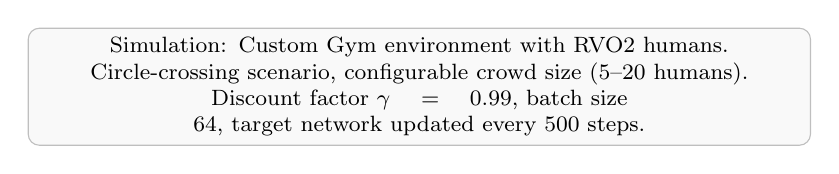
\begin{tikzpicture}
    \node[draw=gray!50, fill=gray!5, rounded corners=4pt,
          font=\footnotesize, text width=0.8\textwidth, align=center] {
      Simulation: Custom Gym environment with RVO2 humans.\\
      Circle-crossing scenario, configurable crowd size (5--20 humans).\\
      Discount factor $\gamma = 0.99$, batch size 64, target network updated every 500 steps.
    };
  \end{tikzpicture}
\end{frame}

% ============================================================
\section{MPC Formulation}
% ============================================================

\begin{frame}{Model Predictive Control: Problem Formulation}
  \begin{block}{Unicycle Dynamics}
    \vspace{-6pt}
    \begin{align}
      x_{k+1} &= x_k + v_k \cos(\theta_k) \cdot \Delta t \nonumber \\
      y_{k+1} &= y_k + v_k \sin(\theta_k) \cdot \Delta t \nonumber \\
      \theta_{k+1} &= \theta_k + \omega_k \cdot \Delta t \nonumber
    \end{align}
  \end{block}

  \vspace{2pt}
  \begin{block}{MPC Optimization}
    \vspace{-4pt}
    \[
      (v^*, \omega^*) = \argmin_{v_{0:N-1},\, \omega_{0:N-1}}
      \sum_{k=0}^{N-1} \underbrace{J_k^{\text{stage}}}_{
        \text{stage cost}} \;+\; \underbrace{J_N^{\text{term}}}_{
        \text{terminal cost}}
    \]
  \end{block}

  \vspace{2pt}
  \textbf{Subject to:}
  \begin{columns}[T]
    \begin{column}{0.45\textwidth}
      \begin{itemize}
        \item $0 \le v_k \le v_{\max}$
        \item $|\omega_k| \le \omega_{\max}$
      \end{itemize}
    \end{column}
    \begin{column}{0.45\textwidth}
      \begin{itemize}
        \item $d_{\text{obs}}(\mathbf{x}_k) \ge d_{\text{hard}}$ \quad (safety)
        \item Unicycle dynamics (above)
      \end{itemize}
    \end{column}
  \end{columns}

  \vspace{6pt}
  \centering
  \footnotesize
  $N = 15$ steps, $\Delta t = 0.2$\,s (horizon = 3.0\,s), 100 random rollouts, 10\,Hz control rate
\end{frame}

% ============================================================
\begin{frame}{MPC Cost Function: Full Breakdown}
  \vspace{-4pt}
  \[
    J_k^{\text{stage}} = \underbrace{J_k^{\text{goal}}}_{\text{\highlight{Goal}}}
    + \underbrace{J_k^{\text{social}}}_{\text{\highlight{SARL Social}}}
    + \underbrace{J_k^{\text{obs}}}_{\text{\mpchl{Obstacle}}}
    + \underbrace{J_k^{\text{smooth}}}_{\text{\mpchl{Smoothness}}}
    + \underbrace{J_k^{\text{vlm}}}_{\text{\vlmhl{VLM}}}
  \]

  \vspace{2pt}
  \begin{columns}[T]
    \begin{column}{0.48\textwidth}
      \textbf{Goal Cost:}
      \[
        J_k^{\text{goal}} = w_g \bigl\|(x_k - g_x,\; y_k - g_y)\bigr\|^2
      \]

      \textbf{SARL Attention-Weighted Social Cost:}
      \[
        J_k^{\text{social}} = \sum_{i=1}^{n}
        \frac{w_s \cdot n \cdot \alpha_i \cdot m_{\text{attn}}}
             {d(\mathbf{x}_k, \mathbf{p}_i) + \epsilon}
      \]
      {\footnotesize where $\alpha_i$ = SARL attention,
       $m_{\text{attn}}$ = scene multiplier}

      \vspace{4pt}
      \textbf{Smoothness Cost:}
      \[
        J_k^{\text{smooth}} = w_{\text{sm}}\bigl[(v_k - v_{k-1})^2 + (\omega_k - \omega_{k-1})^2\bigr]
      \]
    \end{column}

    \begin{column}{0.48\textwidth}
      \textbf{Obstacle Cost:}
      \[
        J_k^{\text{obs}} = \begin{cases}
          +\infty & d < d_{\text{hard}} \\[3pt]
          1000    & d_{\text{hard}} \le d < d_{\min} \\[3pt]
          \dfrac{w_o}{d + 0.1} & d \ge d_{\min}
        \end{cases}
      \]

      \vspace{6pt}
      \textbf{SARL Terminal Cost:}
      \[
        \boxed{J_N^{\text{term}} = -w_t \cdot m_{\text{term}} \cdot V(s_N)}
      \]
      {\footnotesize Negated: higher $V(s)$ $\Rightarrow$ lower cost\\
       $\Rightarrow$ MPC seeks high-value terminal states}
    \end{column}
  \end{columns}
\end{frame}

% ============================================================
\begin{frame}{Random-Shooting MPC with SARL Batch Evaluation}
  \centering
  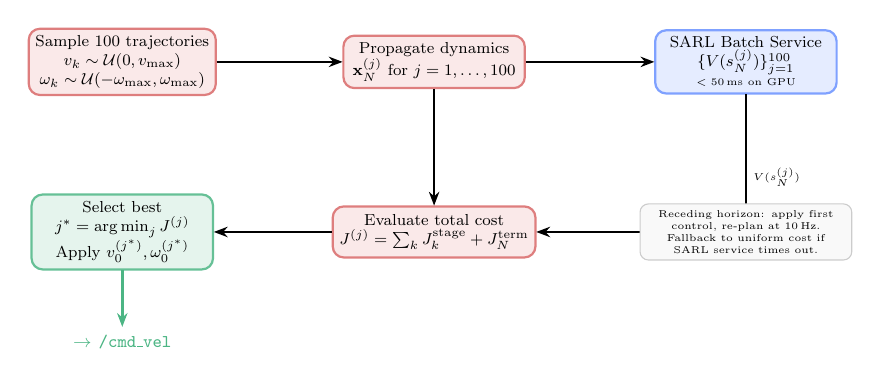
\begin{tikzpicture}[
    scale=0.72, transform shape,
    box/.style={draw, rounded corners=4pt, minimum height=0.9cm,
                align=center, font=\footnotesize, line width=0.8pt},
    proc/.style={box, fill=mpcred!10, draw=mpcred!60, minimum width=3.2cm},
    sarl/.style={box, fill=sarlblue!12, draw=sarlblue!60, minimum width=3.2cm},
    arrow/.style={-{Stealth[length=5pt]}, thick},
  ]
    % Step 1
    \node[proc] (sample) at (0,0) {Sample 100 trajectories\\
      $v_k \sim \mathcal{U}(0, v_{\max})$\\
      $\omega_k \sim \mathcal{U}(-\omega_{\max}, \omega_{\max})$};

    % Step 2
    \node[proc] (prop) at (5.5,0) {Propagate dynamics\\
      $\mathbf{x}_N^{(j)}$ for $j = 1,\dots,100$};

    % Step 3 (SARL batch)
    \node[sarl] (batch) at (11,0) {SARL Batch Service\\
      $\{V(s_N^{(j)})\}_{j=1}^{100}$\\
      {\tiny $< 50$\,ms on GPU}};

    % Step 4
    \node[proc] (eval) at (5.5,-3) {Evaluate total cost\\
      $J^{(j)} = \sum_k J_k^{\text{stage}} + J_N^{\text{term}}$};

    % Step 5
    \node[proc, fill=vlmgreen!10, draw=vlmgreen!60] (best) at (0,-3) {Select best\\
      $j^* = \argmin_j J^{(j)}$\\
      Apply $v_0^{(j^*)}, \omega_0^{(j^*)}$};

    % Arrows
    \draw[arrow] (sample) -- (prop);
    \draw[arrow] (prop) -- (batch);
    \draw[arrow] (batch) |- node[right, font=\tiny, pos=0.3] {$V(s_N^{(j)})$} (eval);
    \draw[arrow] (prop) -- (eval);
    \draw[arrow] (eval) -- (best);

    % Control output
    \draw[arrow, vlmgreen!70, very thick] (best.south) -- ++(0,-1)
      node[below, font=\small\bfseries] {$\to$ \texttt{/cmd\_vel}};

    % Timing annotation
    \node[draw=gray!40, fill=gray!5, rounded corners=3pt,
          font=\tiny, text width=3.5cm, align=center] at (11,-3) {
      Receding horizon: apply first\\
      control, re-plan at 10\,Hz.\\
      Fallback to uniform cost if\\
      SARL service times out.
    };
  \end{tikzpicture}
\end{frame}

% ============================================================
\section{VLM Integration}
% ============================================================

\begin{frame}{Vision-Language Model: Scene Understanding}
\scriptsize
  \begin{columns}[T]
    \begin{column}{0.55\textwidth}
      \textbf{VLM Input (Prompt Assembly):}
      \begin{itemize}
        \item RGB camera image
        \item 3D bounding boxes of detected pedestrians
        \item Robot position and goal
        \item \synhl{SARL attention weights} per person (Synergy~1)
      \end{itemize}

      \vspace{6pt}
      \textbf{VLM Output (Structured):}
      \begin{itemize}
        \item \vlmhl{Scene type}: doorway, corridor, crossing, queue, open\_space
        \item \vlmhl{Crowd density}: empty, sparse, medium, dense
        \item \vlmhl{Recommended action}: go\_ahead, slow\_down, yield, wait
        \item \vlmhl{Confidence}: $[0, 1]$
        \item \vlmhl{Min.\ personal distance}: adaptive threshold
      \end{itemize}

      \vspace{6pt}
      \textbf{Trigger Conditions:}
      \begin{enumerate}
        \item New person detection
        \item Periodic interval (5\,s)
        \item Scene distribution change
      \end{enumerate}
    \end{column}

    \begin{column}{0.42\textwidth}
      \small
      \begin{exampleblock}{\footnotesize Example VLM Prompt (with SARL)}
        \ttfamily\scriptsize
        Robot at (2.1, 3.4), goal (8.0, 1.0)\\[3pt]
        Pedestrians (3):\\
        1. ID=001, Pos=(3.5, 4.1)\\
        \quad Vel=(0.2, -0.1) m/s\\
        \quad \textcolor{synergyorange}{SARL\_ATTN=0.72}\\
        \quad \textcolor{mpcred}{RL\_RISK=HIGH}\\[2pt]
        2. ID=002, Pos=(5.2, 2.8)\\
        \quad Vel=(0.0, 0.3) m/s\\
        \quad \textcolor{synergyorange}{SARL\_ATTN=0.20}\\
        \quad RL\_RISK=LOW\\[2pt]
        3. ID=003, Pos=(1.0, 5.5)\\
        \quad Vel=(-0.1, 0.0) m/s\\
        \quad \textcolor{synergyorange}{SARL\_ATTN=0.08}\\
        \quad RL\_RISK=LOW
      \end{exampleblock}
    \end{column}
  \end{columns}
\end{frame}

% ============================================================
\begin{frame}{VLM Additional Cost Terms for MPC}
  \begin{columns}[T]
    \begin{column}{0.48\textwidth}
      The VLM translator converts semantic outputs into four MPC-compatible cost terms:

      \vspace{6pt}
      \textbf{1. Directional Cost} ($w_{\text{vlm-dir}}$):
      \begin{itemize}
        \item Penalizes heading deviation from VLM-recommended direction
        \item E.g., ``pass on the left''
      \end{itemize}

      \vspace{4pt}
      \textbf{2. Action Cost} ($w_{\text{vlm-act}}$):
      \begin{itemize}
        \item Penalizes velocity when VLM says ``stop and wait'' or ``yield''
      \end{itemize}

      \vspace{4pt}
      \textbf{3. Scene Cost} ($w_{\text{vlm-scene}}$):
      \begin{itemize}
        \item Scene-specific penalties (doorway narrowness, crossing density)
      \end{itemize}

      \vspace{4pt}
      \textbf{4. Personal Space Cost} ($w_{\text{vlm-pers}}$):
      \begin{itemize}
        \item Distance violation when closer than VLM-recommended minimum
      \end{itemize}
    \end{column}

    \begin{column}{0.48\textwidth}
      \begin{block}{VLM Cost in MPC}
        \vspace{-4pt}
        \begin{align*}
          J_k^{\text{vlm}} &= w_{\text{dir}} \cdot C_{\text{dir}}(\theta_k) \\
                           &+ w_{\text{act}} \cdot C_{\text{act}}(v_k) \\
                           &+ w_{\text{scene}} \cdot C_{\text{scene}}(\mathbf{x}_k) \\
                           &+ w_{\text{pers}} \cdot C_{\text{pers}}(d_{\min}^k)
        \end{align*}
      \end{block}

      \vspace{4pt}
      \begin{alertblock}{\footnotesize Enable/Disable VLM}
        \footnotesize
        VLM can be toggled via launch argument \texttt{enable\_vlm}.
        When disabled, MPC uses only SARL attention + standard costs.
        System remains fully functional.
      \end{alertblock}
    \end{column}
  \end{columns}
\end{frame}

% ============================================================
\section{Three Synergy Mechanisms}
% ============================================================

\begin{frame}{Synergy 1: SARL Attention Enriches VLM Prompts}
\scriptsize
  \centering
  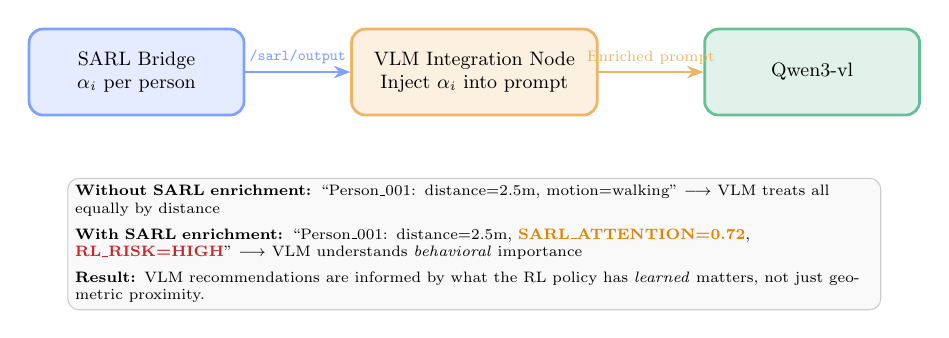
\begin{tikzpicture}[
    scale=0.78, transform shape,
    box/.style={draw, rounded corners=5pt, minimum height=1.4cm,
                align=center, font=\small, line width=1pt},
    arrow/.style={-{Stealth[length=6pt]}, thick},
  ]
    % SARL output
    \node[box, fill=sarlblue!12, draw=sarlblue!60, minimum width=3.5cm]
      (sarl) at (0,0) {SARL Bridge\\$\alpha_i$ per person};

    % VLM Integration
    \node[box, fill=synergyorange!12, draw=synergyorange!60, minimum width=4cm]
      (merge) at (5.5,0) {VLM Integration Node\\Inject $\alpha_i$ into prompt};

    % VLM API
    \node[box, fill=vlmgreen!12, draw=vlmgreen!60, minimum width=3.5cm]
      (vlm) at (11,0) {Qwen3-vl};

    % Arrows
    \draw[arrow, sarlblue!60] (sarl) -- (merge)
      node[midway, above, font=\scriptsize] {\texttt{/sarl/output}};
    \draw[arrow, synergyorange!60] (merge) -- (vlm)
      node[midway, above, font=\scriptsize] {Enriched prompt};

    % Example below
    \node[draw=gray!40, fill=gray!5, rounded corners=4pt,
          font=\scriptsize, text width=13cm, align=left] at (5.5,-2.8) {
      \textbf{Without SARL enrichment:}
      ``Person\_001: distance=2.5m, motion=walking'' $\longrightarrow$
      VLM treats all equally by distance\\[4pt]
      \textbf{With SARL enrichment:}
      ``Person\_001: distance=2.5m, \textcolor{synergyorange}{\textbf{SARL\_ATTENTION=0.72}},
      \textcolor{mpcred}{\textbf{RL\_RISK=HIGH}}'' $\longrightarrow$
      VLM understands \emph{behavioral} importance\\[4pt]
      \textbf{Result:} VLM recommendations are informed by what the RL policy has
      \emph{learned} matters, not just geometric proximity.
    };
  \end{tikzpicture}
\end{frame}

% ============================================================
\begin{frame}{Synergy 2: VLM Scene Context Conditions SARL Weights}
  \begin{columns}[T]
    \begin{column}{0.45\textwidth}
      VLM provides \vlmhl{scene\_type} and \vlmhl{crowd\_density}.\\
      These modulate how much MPC trusts SARL via \texttt{getSceneMultiplier()}:

      \vspace{6pt}
      \[
        J_k^{\text{social}} = \sum_{i}
        \frac{w_s \cdot n \cdot \alpha_i \cdot {\color{synergyorange}\bm{m_{\text{attn}}}}}
             {d_i + \epsilon}
      \]
      \[
        J_N^{\text{term}} = -w_t \cdot {\color{synergyorange}\bm{m_{\text{term}}}} \cdot V(s_N)
      \]

      \vspace{4pt}
      \textbf{Intuition:}
      \begin{itemize}
        \item \textbf{Doorway} (constrained): Amplify SARL $\to$ trust learned social behavior more
        \item \textbf{Open space}: Reduce SARL $\to$ simple distance-based cost suffices
      \end{itemize}
    \end{column}

    \begin{column}{0.52\textwidth}
      \centering
      \textbf{Scene Multiplier Matrix}
      \vspace{4pt}

      \footnotesize
      \begin{tabular}{lcc}
        \toprule
        \textbf{Scene} & $m_{\text{attn}}$ & $m_{\text{term}}$ \\
        \midrule
        Doorway (dense)        & 2.5 & 1.2 \\
        Corridor (dense)       & 2.0 & 1.0 \\
        Corridor (medium)      & 1.5 & 0.7 \\
        Crossing (medium)      & 1.5 & 0.7 \\
        Crossing (sparse)      & 1.0 & 0.5 \\
        Open space (sparse)    & 0.5 & 0.3 \\
        \bottomrule
      \end{tabular}

      \vspace{8pt}
      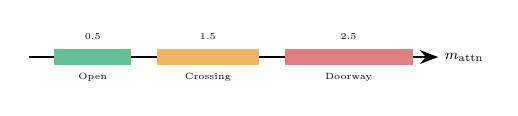
\begin{tikzpicture}[scale=0.65, transform shape]
        \draw[-{Stealth}, thick] (0,0) -- (8,0)
          node[right, font=\footnotesize] {$m_{\text{attn}}$};
        \fill[vlmgreen!60] (0.5,-0.15) rectangle (2,0.15);
        \node[font=\tiny, below] at (1.25,-0.2) {Open};
        \fill[synergyorange!60] (2.5,-0.15) rectangle (4.5,0.15);
        \node[font=\tiny, below] at (3.5,-0.2) {Crossing};
        \fill[mpcred!60] (5,-0.15) rectangle (7.5,0.15);
        \node[font=\tiny, below] at (6.25,-0.2) {Doorway};
        \node[font=\tiny] at (1.25, 0.4) {0.5};
        \node[font=\tiny] at (3.5, 0.4) {1.5};
        \node[font=\tiny] at (6.25, 0.4) {2.5};
      \end{tikzpicture}
    \end{column}
  \end{columns}
\end{frame}

% ============================================================
\begin{frame}{Synergy 3: Combined Interpretability}
  \begin{columns}[T]
    \begin{column}{0.55\textwidth}
      The \texttt{NavigationExplanation} message merges VLM and SARL outputs into
      a \emph{single unified explanation}:

      \vspace{6pt}
      \textbf{Contents:}
      \begin{itemize}
        \item VLM: scene type, crowd density, recommended action, confidence
        \item SARL: per-person attention weights, distances, motion labels
        \item Control: applied $v_{\max}$, $w_{\text{social}}$, scene multiplier
        \item \textbf{Human-readable narrative}
      \end{itemize}

      \vspace{6pt}
      \textbf{Published to:} \texttt{/navigation/explanation}

      \vspace{6pt}
      \begin{exampleblock}{\footnotesize Example Explanation}
        \ttfamily\tiny
        Scene: corridor (medium) | SARL active:\\
        V(s)=0.35, attention\_mult=1.5\\
        Focus: person\_001 (w=0.72, HIGH)\\
        Action: slow\_down | v\_max=0.35 m/s
      \end{exampleblock}
    \end{column}

    \begin{column}{0.42\textwidth}
      \centering
      \textbf{Why Interpretability Matters}

      \vspace{6pt}
      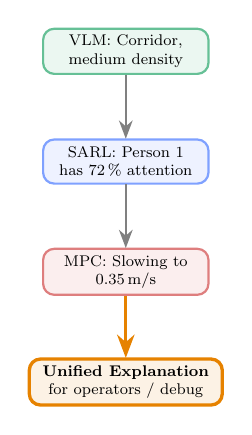
\begin{tikzpicture}[
        scale=0.7, transform shape,
        box/.style={draw, rounded corners=4pt, fill=white,
                    minimum width=3cm, minimum height=0.8cm,
                    align=center, font=\footnotesize, line width=0.8pt},
      ]
        \node[box, draw=vlmgreen!60, fill=vlmgreen!8] (vlm) at (0,4)
          {VLM: Corridor,\\medium density};
        \node[box, draw=sarlblue!60, fill=sarlblue!8] (sarl) at (0,2)
          {SARL: Person 1\\has 72\,\% attention};
        \node[box, draw=mpcred!60, fill=mpcred!8] (mpc) at (0,0)
          {MPC: Slowing to\\0.35\,m/s};

        \draw[-{Stealth}, thick, gray] (vlm) -- (sarl);
        \draw[-{Stealth}, thick, gray] (sarl) -- (mpc);

        \node[box, draw=synergyorange, fill=synergyorange!10,
              minimum width=3.5cm, line width=1.2pt] (exp) at (0,-2)
          {\textbf{Unified Explanation}\\for operators / debug};

        \draw[-{Stealth}, very thick, synergyorange] (mpc) -- (exp);
      \end{tikzpicture}

      \vspace{6pt}
      \footnotesize
      Enables trust calibration, debugging, and human oversight of autonomous navigation decisions.
    \end{column}
  \end{columns}
\end{frame}

% ============================================================
\section{ROS\,2 Implementation}
% ============================================================

\begin{frame}{ROS\,2 Node Architecture}
  \centering
  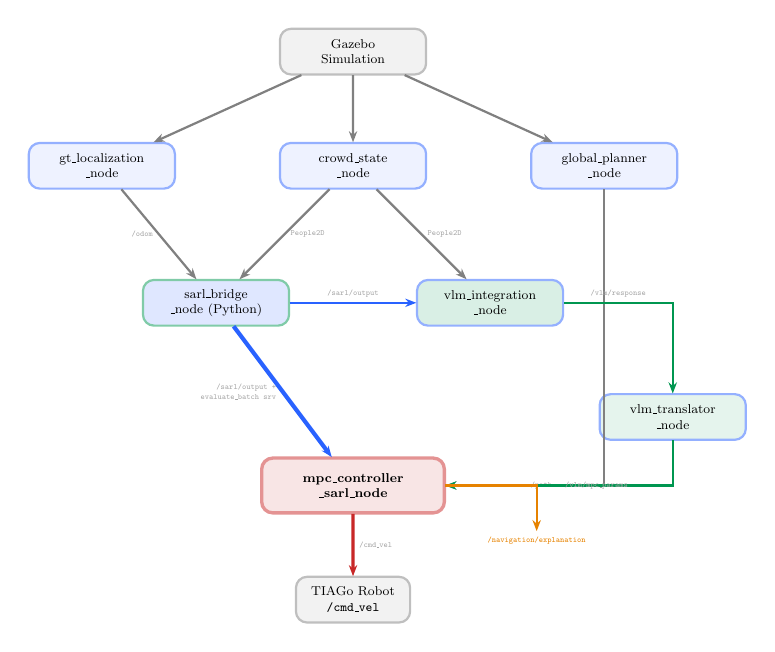
\begin{tikzpicture}[
    scale=0.58, transform shape,
    nodebox/.style={draw, rounded corners=4pt, minimum height=1cm,
                 align=center, font=\footnotesize, line width=0.8pt},
    ros/.style={nodebox, fill=sarlblue!8, draw=sarlblue!50, minimum width=3.2cm},
    py/.style={nodebox, fill=vlmgreen!8, draw=vlmgreen!50, minimum width=3.2cm},
    sim/.style={nodebox, fill=gray!10, draw=gray!50, minimum width=3.2cm},
    topic/.style={font=\tiny\ttfamily, text=gray!70},
    arrow/.style={-{Stealth[length=4pt]}, thick},
  ]
    % Gazebo
    \node[sim] (gaz) at (0,6) {Gazebo\\Simulation};

    % Localization
    \node[ros] (loc) at (-5.5,3.5) {gt\_localization\\\_node};

    % Person tracker
    \node[ros] (pers) at (0,3.5) {crowd\_state\\\_node};

    % Global planner
    \node[ros] (plan) at (5.5,3.5) {global\_planner\\\_node};

    % SARL bridge
    \node[py, fill=sarlblue!15] (sarl) at (-3,0.5) {sarl\_bridge\\\_node (Python)};

    % VLM integration
    \node[ros, fill=vlmgreen!15] (vlm) at (3,0.5) {vlm\_integration\\\_node};

    % VLM translator
    \node[ros, fill=vlmgreen!10] (trans) at (7,-2) {vlm\_translator\\\_node};

    % MPC controller
    \node[ros, fill=mpcred!12, draw=mpcred!50, minimum width=4cm,
          minimum height=1.2cm, line width=1.2pt]
      (mpc) at (0,-3.5) {\textbf{mpc\_controller}\\
        \textbf{\_sarl\_node}};

    % Robot
    \node[sim, minimum width=2.5cm] (robot) at (0,-6) {TIAGo Robot\\\texttt{/cmd\_vel}};

    % Arrows
    \draw[arrow, gray] (gaz) -- (loc);
    \draw[arrow, gray] (gaz) -- (pers);
    \draw[arrow, gray] (gaz) -- (plan);

    \draw[arrow, gray] (loc) -- (sarl) node[midway, left, topic] {/odom};
    \draw[arrow, gray] (pers) -- (sarl) node[midway, right, topic] {People2D};
    \draw[arrow, gray] (pers) -- (vlm) node[midway, right, topic] {People2D};
    \draw[arrow, gray] (plan) |- (mpc) node[near end, right, topic] {/path};

    \draw[arrow, sarlblue] (sarl) -- (vlm)
      node[midway, above, topic] {/sarl/output};
    \draw[arrow, sarlblue, line width=1.5pt] (sarl) -- (mpc)
      node[midway, left, topic, align=right] {/sarl/output +\\ evaluate\_batch srv};

    \draw[arrow, vlmgreen] (vlm) -| (trans)
      node[near start, above, topic] {/vlm/response};
    \draw[arrow, vlmgreen] (trans) |- (mpc)
      node[near end, right, topic] {/vlm/mpc\_params};

    \draw[arrow, mpcred, very thick] (mpc) -- (robot)
      node[midway, right, topic] {/cmd\_vel};

    % Explanation output
    \draw[arrow, synergyorange] (mpc.east) -- ++(2,0) -- ++(0,-1)
      node[below, font=\tiny\ttfamily] {/navigation/explanation};
  \end{tikzpicture}
\end{frame}

% ============================================================
\begin{frame}{SARL Bridge Node: Real-Time Inference}
  \begin{columns}[T]
    \begin{column}{0.48\textwidth}
      \textbf{Dual Interface Design:}

      \vspace{4pt}
      \begin{block}{\footnotesize Interface 1: Topic Publisher (10\,Hz)}
        \begin{itemize}
          \item Subscribes: \texttt{/odom}, \texttt{/person\_info}
          \item Publishes: \texttt{/sarl/output}
          \item Content: $\{\alpha_i\}$, $V(s)$, person IDs
          \item RViz markers: colored spheres\\
                {\scriptsize (green$\to$yellow$\to$red $\propto$ attention)}
        \end{itemize}
      \end{block}

      \begin{block}{\footnotesize Interface 2: Batch Service}
        \begin{itemize}
          \item Service: \texttt{/sarl/evaluate\_batch}
          \item Input: 100 terminal states from MPC
          \item Output: $\{V(s_N^{(j)})\}_{j=1}^{100}$
          \item Latency: $<50$\,ms with PyTorch
        \end{itemize}
      \end{block}
    \end{column}

    \begin{column}{0.48\textwidth}
      \textbf{Implementation Details:}
      \begin{itemize}
        \item Loads \texttt{rl\_model.pth} from CrowdNav
        \item Replicates \texttt{ValueNetwork} architecture exactly
        \item Goal-oriented \texttt{rotate()} coordinate transform
        \item Unicycle $\to$ holonomic velocity conversion:
      \end{itemize}
      \[
        v_x = v \cos(\theta), \quad v_y = v \sin(\theta)
      \]

      \vspace{4pt}
      \textbf{Staleness Handling:}
      \begin{itemize}
        \item SARL data timestamped at publication
        \item MPC checks: if age $> 0.5$\,s $\Rightarrow$ fallback to uniform social cost
        \item Ensures safety even if SARL node crashes
      \end{itemize}

      \vspace{4pt}
      \textbf{RViz Attention Markers:}
      \begin{itemize}
        \item Sphere radius: $0.2 + \alpha_i \times 0.6$\,m
        \item Text label: person ID + attention weight
        \item $V(s)$ displayed above robot
      \end{itemize}
    \end{column}
  \end{columns}
\end{frame}

% ============================================================
\begin{frame}{Social Contract Helper: Rule-Based Safety Layer}
\scriptsize
  \begin{columns}[T]
    \begin{column}{0.5\textwidth}
      \textbf{Purpose:} Proximity-based heuristic that adjusts MPC parameters
      \emph{before} optimization, providing an additional safety layer on top
      of SARL attention.

      \vspace{6pt}
      \textbf{Adjustable Parameters:}
      \begin{itemize}
        \item $v_{\max}$: reduced when people nearby
        \item $w_{\text{social}}$: increased when person in path
        \item $d_{\min}^{\text{person}}$: minimum distance threshold
        \item \texttt{person\_in\_front}: boolean flag for blocking detection
      \end{itemize}

      \vspace{6pt}
      \textbf{Integration with SARL:}
      \begin{itemize}
        \item Social contract sets \emph{baseline} $w_{\text{social}}$
        \item SARL attention \emph{redistributes} this weight across pedestrians
        \item VLM scene multiplier \emph{scales} the combined result
      \end{itemize}
    \end{column}

    \begin{column}{0.45\textwidth}
      \centering
      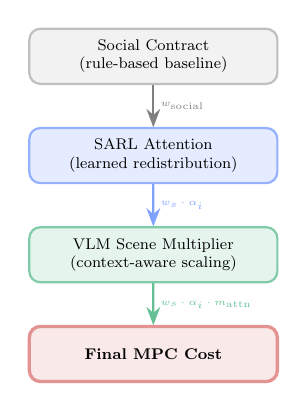
\begin{tikzpicture}[
        scale=0.7, transform shape,
        layer/.style={draw, rounded corners=4pt, minimum width=4.5cm,
                      minimum height=1cm, align=center, font=\footnotesize,
                      line width=0.8pt},
      ]
        \node[layer, fill=gray!10, draw=gray!50] (sc) at (0,3)
          {Social Contract\\(rule-based baseline)};
        \node[layer, fill=sarlblue!12, draw=sarlblue!50] (sarl) at (0,1.2)
          {SARL Attention\\(learned redistribution)};
        \node[layer, fill=vlmgreen!10, draw=vlmgreen!50] (vlm) at (0,-0.6)
          {VLM Scene Multiplier\\(context-aware scaling)};
        \node[layer, fill=mpcred!10, draw=mpcred!50, line width=1.2pt]
          (mpc) at (0,-2.4)
          {\textbf{Final MPC Cost}};

        \draw[-{Stealth}, thick, gray] (sc) -- (sarl)
          node[midway, right, font=\tiny] {$w_{\text{social}}$};
        \draw[-{Stealth}, thick, sarlblue!60] (sarl) -- (vlm)
          node[midway, right, font=\tiny] {$w_s \cdot \alpha_i$};
        \draw[-{Stealth}, thick, vlmgreen!60] (vlm) -- (mpc)
          node[midway, right, font=\tiny] {$w_s \cdot \alpha_i \cdot m_{\text{attn}}$};
      \end{tikzpicture}
    \end{column}
  \end{columns}
\end{frame}

% ============================================================
\section{Configuration \& Deployment}
% ============================================================

\begin{frame}{Key Configuration Parameters}
  \begin{columns}[T]
    \begin{column}{0.48\textwidth}
      \begin{block}{\footnotesize MPC Parameters (\texttt{mpc\_sarl.yaml})}
        \footnotesize
        \begin{tabular}{lrl}
          \toprule
          \textbf{Parameter} & \textbf{Value} & \textbf{Unit} \\
          \midrule
          $\Delta t$        & 0.2     & s \\
          $N$ (horizon)     & 15      & steps \\
          Rollouts          & 100     & --- \\
          Control rate      & 10      & Hz \\
          \midrule
          $w_{\text{goal}}$    & 2.0  & --- \\
          $w_{\text{social}}$  & 1.0  & --- \\
          $w_{\text{obstacle}}$& 3.0  & --- \\
          $w_{\text{smooth}}$  & 0.1  & --- \\
          \midrule
          $w_{\text{sarl-attn}}$    & 1.0 & --- \\
          $w_{\text{sarl-term}}$    & 0.5 & --- \\
          Staleness timeout         & 0.5 & s \\
          \midrule
          $d_{\text{hard}}$    & 0.2  & m \\
          $d_{\min}^{\text{obs}}$ & 0.3 & m \\
          \bottomrule
        \end{tabular}
      \end{block}
    \end{column}

    \begin{column}{0.48\textwidth}
      \begin{block}{\footnotesize SARL Bridge (\texttt{sarl\_bridge.yaml})}
        \footnotesize
        \begin{tabular}{ll}
          \toprule
          \textbf{Parameter} & \textbf{Value} \\
          \midrule
          Model path   & \texttt{rl\_model.pth} \\
          MLP$_1$ dims & [150, 100] \\
          MLP$_2$ dims & [100, 50] \\
          MLP$_3$ dims & [150,100,100,1] \\
          Attn dims    & [100, 100, 1] \\
          Global state & True \\
          Publish rate  & 10\,Hz \\
          \bottomrule
        \end{tabular}
      \end{block}

      \vspace{4pt}
      \begin{exampleblock}{\footnotesize Launch Command}
        \ttfamily\tiny
        ros2 launch social\_mpc\_nav \\
        \quad mpc\_sarl\_vlm.launch.py \\
        \quad enable\_vlm:=true \\
        \quad log\_mpc\_to\_csv:=true \\
        \quad goal\_x:=10.0 goal\_y:=5.0
      \end{exampleblock}
    \end{column}
  \end{columns}
\end{frame}

% ============================================================
\section{Algorithm Summary}
% ============================================================

\begin{frame}{VISTA-MPC + SARL: Complete Algorithm}
\scriptsize
  \begin{columns}[T]
    \begin{column}{0.55\textwidth}
      \begin{algorithmic}[1]
        \footnotesize
        \REQUIRE Trained SARL model, VLM API, MPC config
        \STATE \textbf{Initialize} ROS\,2 nodes, load SARL weights
        \WHILE{navigation active (at 10\,Hz)}
          \STATE Get robot state $(x, y, \theta, v)$ from odometry
          \STATE Get pedestrian states $\lbrace\mathbf{p}_i, \mathbf{v}_i\rbrace$ from tracker
          \STATE \textcolor{sarlblue}{\textbf{// SARL Inference (10\,Hz)}}
          \STATE Rotate states to goal-centric frame
          \STATE Compute $\lbrace\alpha_i\rbrace, V(s)$ via ValueNetwork
          \STATE Publish \texttt{/sarl/output}
          \STATE \textcolor{vlmgreen}{\textbf{// VLM (event-triggered)}}
          \IF{trigger condition met}
            \STATE Assemble prompt with SARL $\alpha_i$ \hfill \textit{Syn.\,1}
            \STATE Query VLM $\to$ scene type, density, action
          \ENDIF
          \STATE \textcolor{mpcred}{\textbf{// MPC Optimization}}
          \STATE Get scene multiplier $m_{\text{attn}}, m_{\text{term}}$ \hfill \textit{Syn.\,2}
          \STATE Sample 100 random trajectories
          \STATE Call \texttt{evaluate\_batch} $\to \lbrace V(s_N^{(j)})\rbrace$
          \STATE Evaluate $J^{(j)}$ with all cost terms
          \STATE $j^* \gets \argmin_j J^{(j)}$
          \STATE Apply $v_0^{(j^*)}, \omega_0^{(j^*)}$ to \texttt{/cmd\_vel}
          \STATE Publish explanation \hfill \textit{Syn.\,3}
        \ENDWHILE
      \end{algorithmic}
    \end{column}

    \begin{column}{0.42\textwidth}
      \vspace{8pt}
      \textbf{Key Properties:}
      \begin{itemize}
        \item[\textcolor{sarlblue}{\scriptsize$\blacksquare$}] \textbf{Anytime:} Best trajectory available at any point
        \item[\textcolor{vlmgreen}{\scriptsize$\blacksquare$}] \textbf{Graceful degradation:} VLM timeout $\to$ SARL-only; SARL stale $\to$ uniform cost
        \item[\textcolor{mpcred}{\scriptsize$\blacksquare$}] \textbf{Safety:} Hard distance constraints always enforced
        \item[\textcolor{synergyorange}{\scriptsize$\blacksquare$}] \textbf{Interpretable:} Every decision is explainable
      \end{itemize}

      \vspace{10pt}
      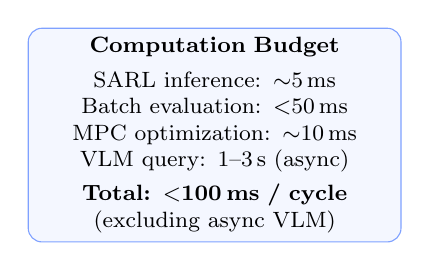
\begin{tikzpicture}
        \node[draw=sarlblue!60, fill=sarlblue!5, rounded corners=5pt,
              font=\footnotesize, text width=4.5cm, align=center] {
          \textbf{Computation Budget}\\[3pt]
          SARL inference: $\sim$5\,ms\\
          Batch evaluation: $<$50\,ms\\
          MPC optimization: $\sim$10\,ms\\
          VLM query: 1--3\,s (async)\\[3pt]
          \textbf{Total: $<$100\,ms / cycle}\\
          (excluding async VLM)
        };
      \end{tikzpicture}
    \end{column}
  \end{columns}
\end{frame}

% ============================================================
\section{Discussion \& Conclusion}
% ============================================================

\begin{frame}{Key Contributions}
  \begin{enumerate}
    \item \textbf{Hierarchical VLM--SARL--MPC integration}\\
      First framework combining learned social attention, vision-language scene understanding,
      and model predictive control in a principled three-layer hierarchy.

    \vspace{6pt}
    \item \textbf{Three synergy mechanisms}\\
      \begin{itemize}
        \item[\synhl{S1}] SARL attention enriches VLM prompts for better scene analysis
        \item[\synhl{S2}] VLM scene context adaptively scales SARL cost contributions
        \item[\synhl{S3}] Combined interpretability for human-readable navigation explanations
      \end{itemize}

    \vspace{6pt}
    \item \textbf{SARL terminal value for MPC}\\
      Learned value function $V(s_N)$ provides long-horizon social reasoning
      beyond MPC's finite horizon (3\,s), evaluated in batch for 100 rollouts.

    \vspace{6pt}
    \item \textbf{Robust real-time system}\\
      ROS\,2 implementation with graceful fallback (SARL stale $\to$ uniform cost),
      hard safety constraints, and full CSV logging for experiment analysis.
  \end{enumerate}
\end{frame}

% ============================================================
\begin{frame}{Advantages of the Hybrid Approach}
  \centering
  \footnotesize
  \begin{tabular}{p{2.8cm}ccc}
    \toprule
    \textbf{Property} &
    \textbf{Pure RL} &
    \textbf{Pure MPC} &
    \textbf{VISTA-MPC+SARL} \\
    \midrule
    Social attention &
    \textcolor{vlmgreen}{$\checkmark$} &
    \textcolor{mpcred}{$\times$} &
    \textcolor{vlmgreen}{$\checkmark$} \\[3pt]

    Scene understanding &
    \textcolor{mpcred}{$\times$} &
    \textcolor{mpcred}{$\times$} &
    \textcolor{vlmgreen}{$\checkmark$} (VLM) \\[3pt]

    Safety guarantees &
    \textcolor{mpcred}{$\times$} &
    \textcolor{vlmgreen}{$\checkmark$} &
    \textcolor{vlmgreen}{$\checkmark$} \\[3pt]

    Interpretability &
    \textcolor{mpcred}{$\times$} &
    \textcolor{synergyorange}{$\sim$} &
    \textcolor{vlmgreen}{$\checkmark$} \\[3pt]

    Long-horizon reasoning &
    \textcolor{vlmgreen}{$\checkmark$} ($V(s)$) &
    \textcolor{synergyorange}{$\sim$} (finite $N$) &
    \textcolor{vlmgreen}{$\checkmark$} (both) \\[3pt]

    Scene adaptation &
    Fixed policy &
    Manual tuning &
    \textcolor{vlmgreen}{Automatic} \\[3pt]

    Graceful fallback &
    \textcolor{mpcred}{$\times$} &
    \textcolor{vlmgreen}{$\checkmark$} &
    \textcolor{vlmgreen}{$\checkmark$} \\
    \bottomrule
  \end{tabular}

  \vspace{12pt}
  
\begin{tikzpicture}
    \node[draw=sarlblue, fill=sarlblue!5, rounded corners=6pt,
          text width=0.8\textwidth, align=center, font=\small,
          line width=1pt] {
      VISTA-MPC + SARL combines the \textbf{social intelligence} of deep RL,\\
      the \textbf{semantic reasoning} of VLMs, and the
      \textbf{safety \& optimality} of MPC.
    };
  \end{tikzpicture}
\end{frame}

% ============================================================
\begin{frame}{Future Work}
  \begin{columns}[T]
    \begin{column}{0.48\textwidth}
      \begin{block}{Short-Term}
        \begin{itemize}
          \item Real robot deployment on TIAGo platform
          \item Systematic ablation study:\\ VLM-only vs SARL-only vs combined
          \item Human-subject evaluation of social compliance
          \item Benchmark on standard SocNav datasets
        \end{itemize}
      \end{block}
    \end{column}

    \begin{column}{0.48\textwidth}
      \begin{block}{Long-Term}
        \begin{itemize}
          \item End-to-end fine-tuning of SARL with VLM feedback
          \item Pedestrian trajectory prediction integration
          \item Multi-robot coordination with shared attention
          \item CasADi-based gradient MPC replacing random shooting
          \item Smaller on-device VLMs for edge deployment
        \end{itemize}
      \end{block}
    \end{column}
  \end{columns}


  \vspace{6pt}
  \footnotesize
  Code: \texttt{github.com/huojiaxi/RL-Social-Nav}
\end{frame}

% ============================================================
% APPENDIX
% ============================================================
\appendix

\begin{frame}[noframenumbering]{Appendix: Message Definitions}
  \begin{columns}[T]
    \begin{column}{0.32\textwidth}
      \begin{block}{\footnotesize SARLOutput.msg}
        \ttfamily\tiny
        time stamp\\
        float32[] attention\_weights\\
        string[] person\_names\\
        float32 state\_value\\
        float32 robot\_x\\
        float32 robot\_y\\
        float32 robot\_yaw\\
        float32 inference\_time\_ms\\
        bool is\_valid
      \end{block}
    \end{column}

    \begin{column}{0.32\textwidth}
      \begin{block}{\footnotesize EvaluateSARLBatch.srv}
        \ttfamily\tiny
        \# Request\\
        float32[] robot\_states\\
        float32 goal\_x\\
        float32 goal\_y\\
        float32[] people\_states\\
        int32 num\_rollouts\\
        int32 num\_people\\
        ---\\
        \# Response\\
        float32[] values\\
        float32 inference\_time\_ms\\
        bool success
      \end{block}
    \end{column}

    \begin{column}{0.32\textwidth}
      \begin{block}{\footnotesize NavigationExplanation}
        \ttfamily\tiny
        string scene\_type\\
        string crowd\_density\\
        string recommended\_action\\
        float32 vlm\_confidence\\
        string[] person\_names\\
        float32[] attention\_weights\\
        float32[] person\_distances\\
        string[] person\_motions\\
        float32 state\_value\\
        float32 applied\_v\_max\\
        float32 applied\_w\_social\\
        float32 sarl\_scene\_mult\\
        string explanation\_text
      \end{block}
    \end{column}
  \end{columns}
\end{frame}

% ============================================================
\begin{frame}[noframenumbering]{Appendix: SARL Network Dimensions}
  \centering
  \footnotesize
  \begin{tabular}{llccc}
    \toprule
    \textbf{Component} & \textbf{Layer} & \textbf{Input} & \textbf{Output} & \textbf{Activation} \\
    \midrule
    \multirow{2}{*}{MLP$_1$ (Encoder)}
      & Linear + ReLU & 13   & 150 & ReLU \\
      & Linear + ReLU & 150  & 100 & ReLU \\
    \midrule
    \multirow{3}{*}{Attention MLP}
      & Linear + ReLU & 200  & 100 & ReLU \\
      & Linear + ReLU & 100  & 100 & ReLU \\
      & Linear        & 100  & 1   & --- \\
    \midrule
    MLP$_2$ (Features)
      & Linear + ReLU & 100  & 50  & ReLU \\
    \midrule
    \multirow{4}{*}{MLP$_3$ (Value Head)}
      & Linear + ReLU & 56   & 150 & ReLU \\
      & Linear + ReLU & 150  & 100 & ReLU \\
      & Linear + ReLU & 100  & 100 & ReLU \\
      & Linear        & 100  & 1   & --- \\
    \bottomrule
  \end{tabular}

  \vspace{12pt}
  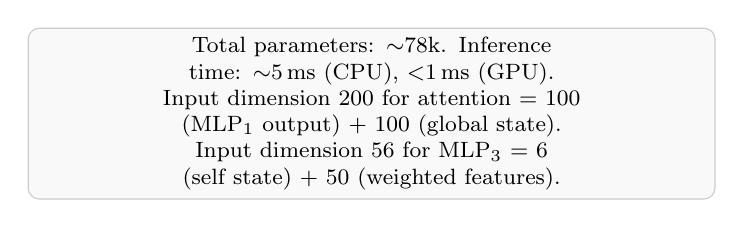
\begin{tikzpicture}
    \node[draw=gray!40, fill=gray!5, rounded corners=4pt,
          font=\footnotesize, text width=0.7\textwidth, align=center] {
      Total parameters: $\sim$78k. Inference time: $\sim$5\,ms (CPU), $<$1\,ms (GPU).\\
      Input dimension 200 for attention = 100 (MLP$_1$ output) + 100 (global state).\\
      Input dimension 56 for MLP$_3$ = 6 (self state) + 50 (weighted features).
    };
  \end{tikzpicture}
\end{frame}

\begin{frame}{VISTA-MPC with SARL}
    \begin{figure}
        \centering
        \includegraphics[width=\linewidth]{pics/Screenshot from 2026-01-29 08-00-23.png}
        % \caption{Caption}
        % \label{fig:placeholder}
    \end{figure}
\end{frame}

\begin{frame}{VISTA-MPC with SARL}
    \begin{figure}
        \centering
        \includegraphics[width=\linewidth]{pics/Screenshot from 2026-01-29 08-02-29.png}
        % \caption{Caption}
        % \label{fig:placeholder}
    \end{figure}
\end{frame}

\begin{frame}{VISTA-MPC with SARL}
    \begin{figure}
        \centering
        \includegraphics[width=\linewidth]{pics/Screenshot from 2026-01-29 08-11-09.png}
        % \caption{Caption}
        % \label{fig:placeholder}
    \end{figure}
\end{frame}



\end{document}
